\documentclass[border=6pt]{standalone}
\usepackage{fontspec,unicode-math}
\setmainfont{Noto Serif}
\setmathfont{STIXTwoMath-Regular.otf}
\usepackage{tikz}
\usetikzlibrary{arrows.meta,calc,patterns,decorations.pathmorphing}
\tikzset{heavy/.style={line width=1.1pt,line cap=round,line join=round},
 fine/.style={line width=.58pt,line cap=round,line join=round},
 pale/.style={line width=.40pt},
 arr/.style={line width=.70pt,-{Latex[length=1.9mm,width=1.1mm]}},
 dim/.style={line width=.58pt,{Latex[length=1.55mm,width=.85mm]}-{Latex[length=1.55mm,width=.85mm]}},
 txt/.style={font=\fontsize{11}{13}\selectfont,inner sep=1.1pt},
 mini/.style={font=\fontsize{9}{11}\selectfont,inner sep=.9pt}}
\begin{document}
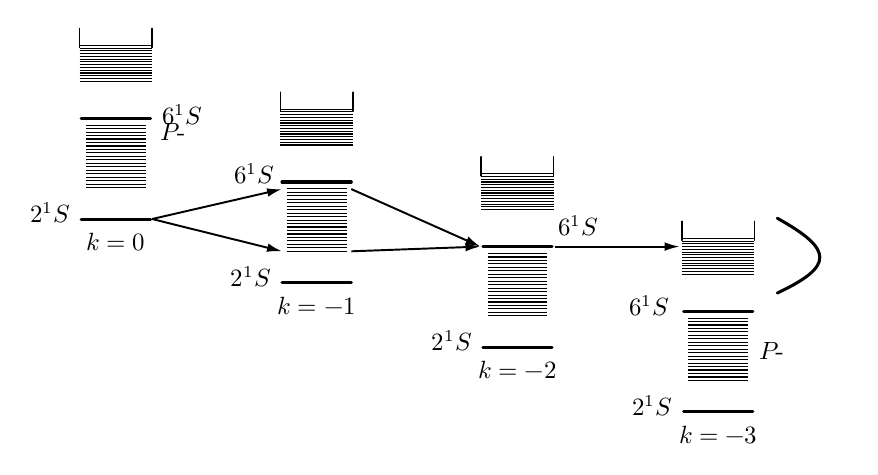
\begin{tikzpicture}[x=1cm,y=1cm]
% Column positions are diagrammatic; the horizontal axis is Floquet index, not energy.
\foreach \x/\k/\y in {0.7/0/3.04,3.25/{-1}/2.23,5.8/{-2}/1.41,8.35/{-3}/.59}{
  \draw[heavy] (\x-.44,\y)--(\x+.44,\y);
  \node[mini,anchor=north] at (\x,\y-.14) {$k=\k$};
  \node[mini,anchor=east] at (\x-.56,\y+.08) {$2{}^1S$};
  \draw[heavy] (\x-.44,\y+1.28)--(\x+.44,\y+1.28);

  % Broad continuum above 6S, separated by a visible gap.
  \foreach \j in {0,...,13}{\draw[pale] (\x-.46,\y+1.75+.035*\j)--(\x+.46,\y+1.75+.035*\j);}
  \draw[fine] (\x-.46,\y+2.18)--(\x-.46,\y+2.42);
  \draw[fine] (\x+.46,\y+2.18)--(\x+.46,\y+2.42);
  % Intermediate P levels, not a claim of the precise helium term energies.
  \foreach \j in {0,...,18}{\draw[pale] (\x-.38,\y+.40+.044*\j)--(\x+.38,\y+.40+.044*\j);}
}
\node[mini,anchor=west,fill=white,inner sep=1pt] at (1.23,4.14) {$P$-состояния};
\node[mini,anchor=west] at (1.25,4.37) {$6{}^1S$};
\node[mini,anchor=east] at (2.73,3.61) {$6{}^1S$};
\node[mini,anchor=west] at (6.28,2.95) {$6{}^1S$};
\node[mini,anchor=east] at (7.75,1.94) {$6{}^1S$};
\node[mini,anchor=west,fill=white,inner sep=1pt] at (8.83,1.36) {$P$-состояния};
% Explicit one-photon arrows; no endpoints silently attach to the wrong manifold.
\coordinate (s) at (1.16,3.04);
\coordinate (p1a) at (2.81,3.42); \coordinate (p1b) at (2.81,2.63);
\draw[arr] (s)--(p1a);\draw[arr] (s)--(p1b);
\draw[arr] (3.69,3.42)--(5.33,2.69);\draw[arr] (3.69,2.63)--(5.33,2.69);
\draw[arr] (6.28,2.69)--(7.86,2.69);
% Original's right-hand outward, unlabeled continuum characteristic.
\draw[heavy] (9.10,2.1) .. controls (9.82,2.44) and (9.82,2.65) .. (9.10,3.05);
\end{tikzpicture}
\end{document}
